\documentclass{article}

% these packages let you do math
\usepackage{amsmath}
\usepackage{amssymb}

% we need these packages for fancy R tables
\usepackage{booktabs}
\usepackage{float}
\usepackage{colortbl}
\usepackage{xcolor}

% these packages play with the spacing/margins of the document. Uncomment the commands on lines 16 and 17 to see what they do.
\usepackage{a4wide}
\usepackage{setspace}
\usepackage{geometry}
\usepackage{parskip}
%\doublespacing
%\geometry{margin=1.5in}

% this package helps us with including images. Setting the graphics path makes it easier to refer to things in the \includegraphics command.
\usepackage{graphicx}
\graphicspath{ {../figures/} }

% make some hyperlinks using the \href command
\usepackage{hyperref}
\hypersetup{
    colorlinks=true,
    linkcolor=black,
    urlcolor=blue
}

% set the author, title, and date of the document. \maketitle adds it to the document.
\author{John Bowman}
\title{My Paper on NLSY97 Data}
\date{Sping 2022}

\begin{document}
\maketitle

\section{Outline}

In this brief study, I tabulated the incarceration status of individuals who responded to the National Longitudinal Survey of Youth in 2002. Using this information, I made a model to predict incarceration status based on racial and gender identity.

The survey collects data on the incarceration status of an individual by month. For the purpose of this study, I generated a  binary indicator variable of whether this individual was incarcerated at any point during the year. The survey also collects racial and gender data. The racial categories are Black, Hispanic, Mixed Race Non Hispanic, and Non Black Non Hispanic.


$$
    Incarcerated = race\beta + gender\beta + \varepsilon
$$

The model above predicts the probability of incarceration, based on race and gender. Because each variable is an indicator variable only one race and gender status is assigned to a given observation and is associated with a multiplicative change in probability.

\newpage

\section{Analysis}

The \texttt{figure} below visualizes the count of individuals who are incarcerated split up by the aforementioned gender and racial groups. It should be noted that the survey includes responses from 8,621 individuals, but there are only a total of 178 displayed in the graph and counted in the subsequent table. Additionally, there are no observations of incarceration for Mixed Race Non Hispanic Males. This will likely cause distortions in the regression since the sample of individuals who are actually incarcerated is simply not large enough for an accurate probability estimate of incarceration. 


\begin{figure}[H]
    \begin{center}
        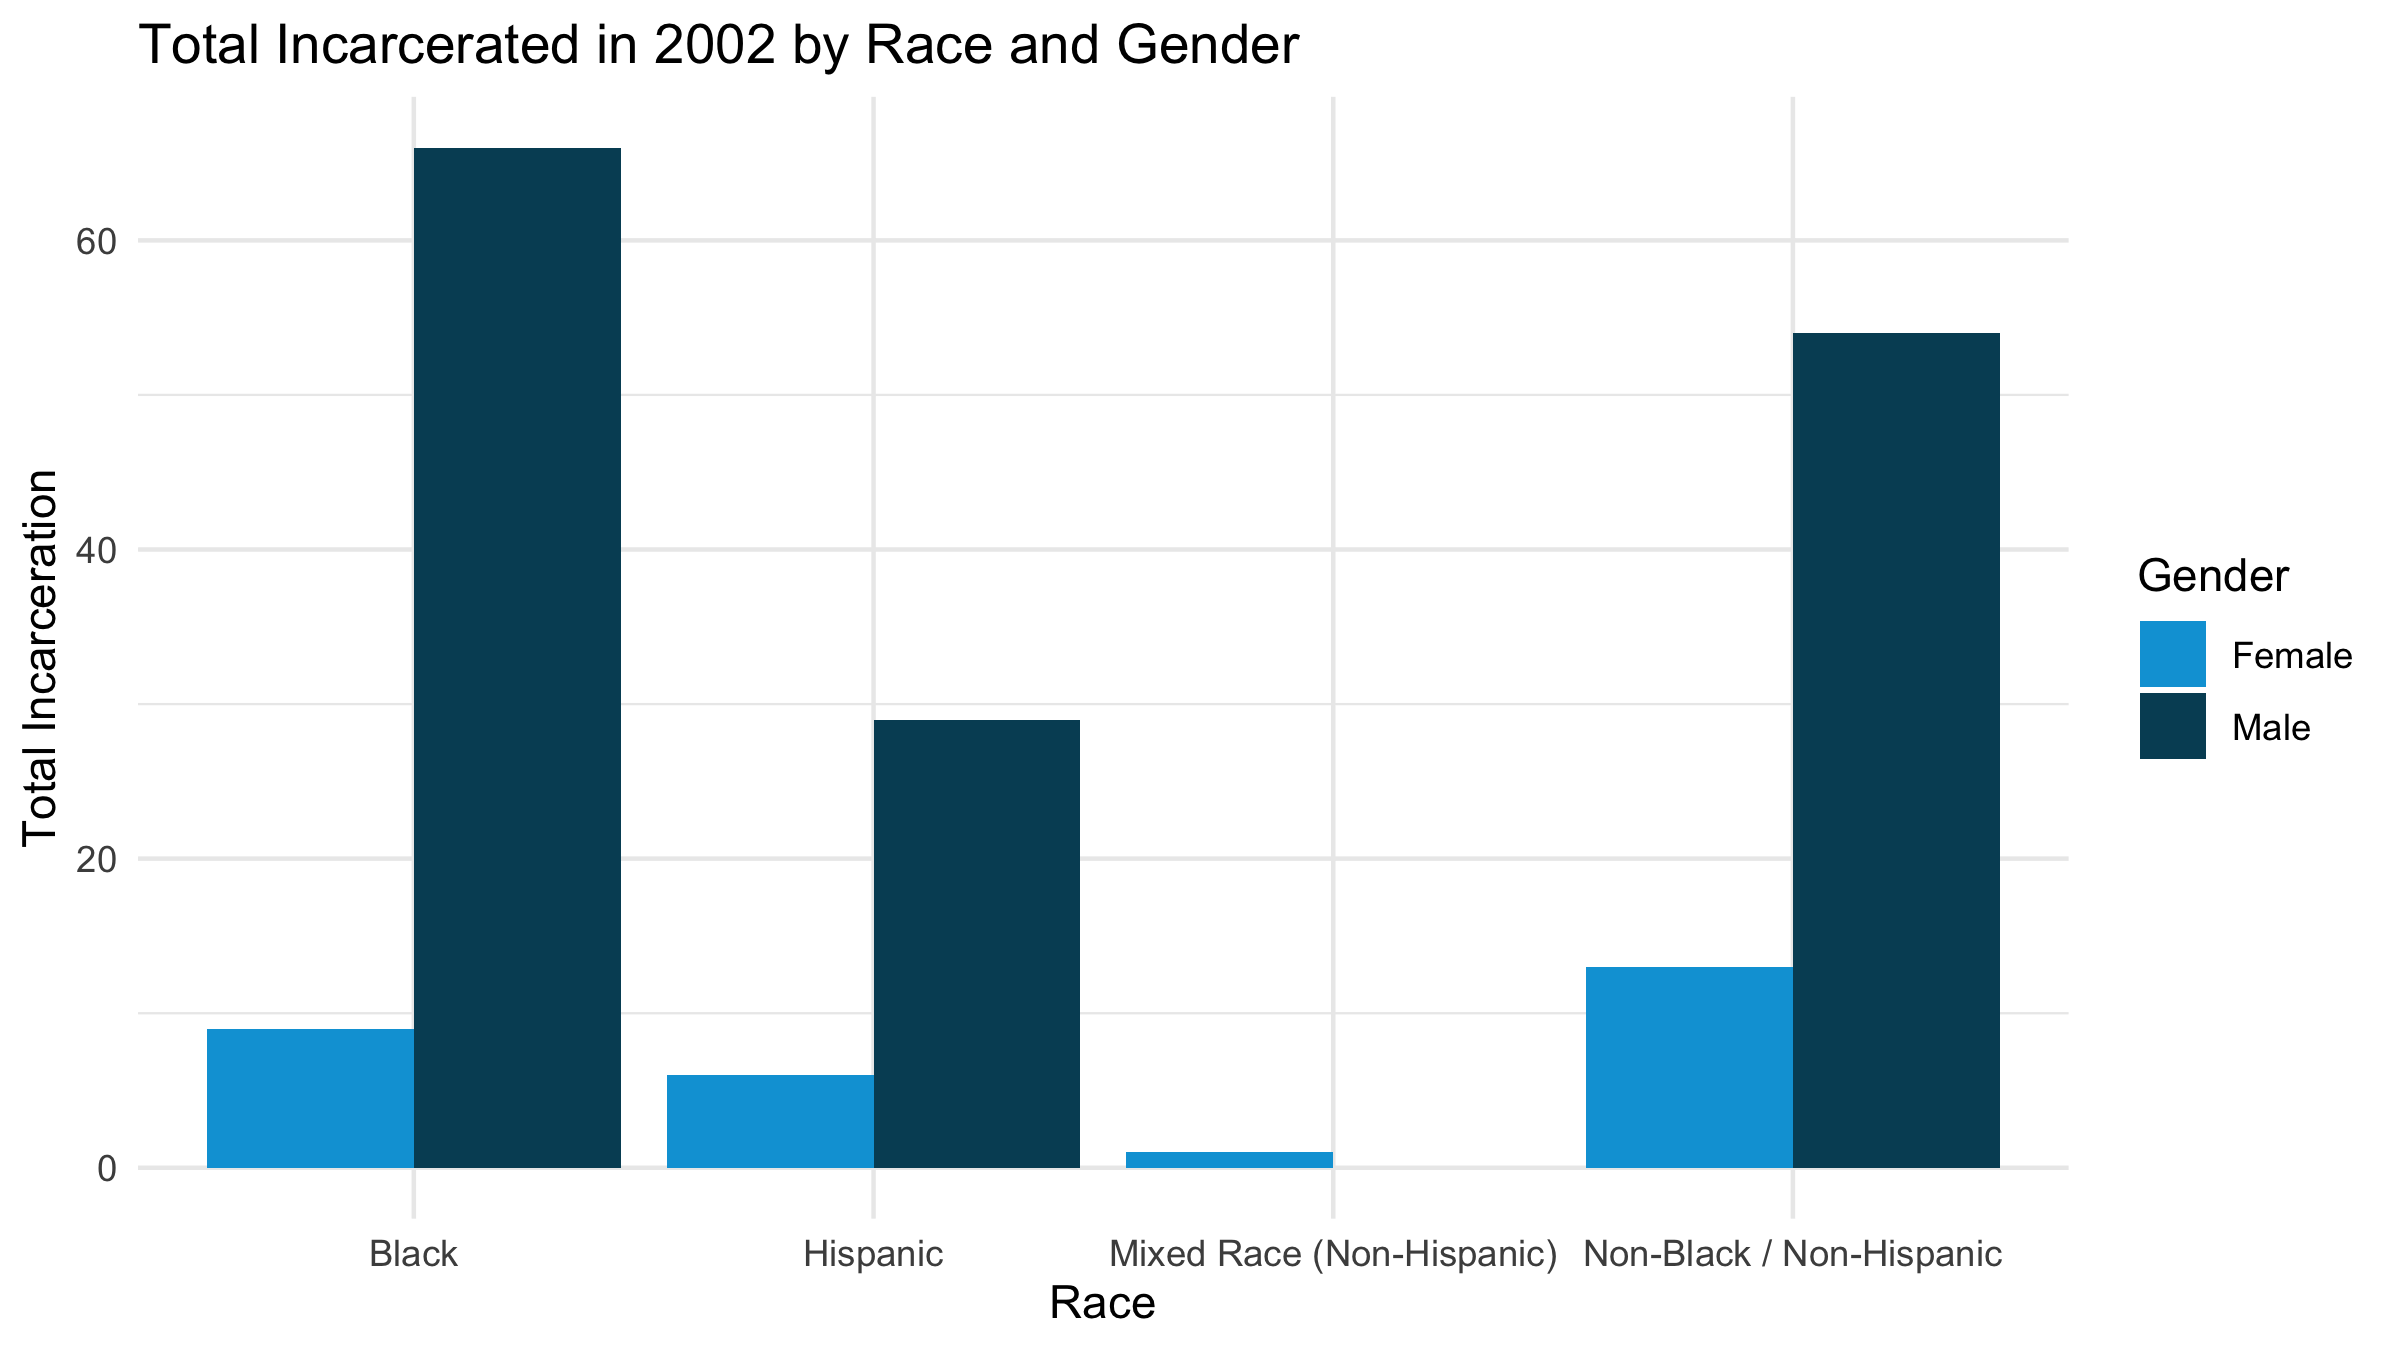
\includegraphics[width=.85\textwidth]{../figures/incarcerated_by_racegender.png}
    \end{center}
    \caption{Mean Number of Months Incarcerated in 2002 by Race and Gender (this is the LaTeX caption, not the ggplot title)}
    \label{fig:graph}
\end{figure}


Figure \ref{fig:graph} does demonstrate some expected qualites. Males are vastly over represented in terms of incarceration status. Ethnic minorites are also overrepresented, compared to the per capita population. The causal relationships for these outcomes are not the subject of this study, but they deserve merit as they could indicate systemic inequites in the justice system. The \texttt{table} below represent the above bar plot numerically.

\begin{table}[H]

\caption{\label{tab:tab:summarystats}Months incarcerated in 2002 by Race and Gender}
\centering
\begin{tabular}[t]{lrrrr}
\toprule
Gender & Black & Hispanic & Mixed Race Non Hispanic & Non Black Non Hispanic\\
\midrule
\cellcolor{gray!6}{Female} & \cellcolor{gray!6}{9} & \cellcolor{gray!6}{6} & \cellcolor{gray!6}{1} & \cellcolor{gray!6}{13}\\
Male & 66 & 29 & 0 & 54\\
\bottomrule
\end{tabular}
\end{table}



% Table created by stargazer v.5.2.2 by Marek Hlavac, Harvard University. E-mail: hlavac at fas.harvard.edu
% Date and time: Wed, Feb 16, 2022 - 20:43:53
\begin{table}[!htbp] \centering 
  \caption{Regression Output. Omitted category is Black Females.} 
  \label{tab:regression} 
\begin{tabular}{@{\extracolsep{5pt}}lc} 
\\[-1.8ex]\hline 
\hline \\[-1.8ex] 
 & \multicolumn{1}{c}{\textit{Dependent variable:}} \\ 
\cline{2-2} 
\\[-1.8ex] & Incarceration status in 2002 \\ 
\hline \\[-1.8ex] 
 Hispanic & $-$0.618$^{***}$ \\ 
  & (0.209) \\ 
  & \\ 
 Mixed Race (Non-Hispanic) & $-$1.021 \\ 
  & (1.036) \\ 
  & \\ 
 Non-Black / Non-Hispanic & $-$0.866$^{***}$ \\ 
  & (0.172) \\ 
  & \\ 
 Male & 1.660$^{***}$ \\ 
  & (0.205) \\ 
  & \\ 
 Constant & $-$4.470$^{***}$ \\ 
  & (0.197) \\ 
  & \\ 
\hline \\[-1.8ex] 
Observations & 8,621 \\ 
Log Likelihood & $-$810.209 \\ 
Akaike Inf. Crit. & 1,630.419 \\ 
\hline 
\hline \\[-1.8ex] 
\textit{Note:}  & \multicolumn{1}{r}{$^{*}$p$<$0.1; $^{**}$p$<$0.05; $^{***}$p$<$0.01} \\ 
\end{tabular} 
\end{table} 


To interpret these results, take e to the power of the beta value, the probability is multiplied by this exponent. These results show negative probability  across the board, with the exception of male. It is likely that the negative probability  are due to a overwhelming number of individuals in the data set who were not incarcerated. It is likely that this data set is not large enough to properly predict these probability.

\end{document}
